\section{Ergebnisse}

\todoAll{Ergebnisse (wertungsfrei) beschreiben}

Unsere Studie wurde vom 04. Juni bis zum 18. August 2019 durchgeführt. Es nahmen insgesamt 45 Teilnehmer in zwei Durchläufen teil. Der erste Durchlauf erfasste zwei Gruppen, dessen geänderter Parameter die Zeit war, in der ein Licht innerhalb der virtuellen Umgebung die Probanden 'geweckt' hat. Im zweiten Durchlauf wurde dieser Parameter geändert und die Teilnehmer wurden mit einem Ton geweckt, wie man ihn als Hinweiston in modernen Autos wiederfindet. Hierbei wurde die Zeit, in der die Studienteilnehmer den Ton selbständig abgeschaltet haben gemessen. Zusätzlich zur Interaktionen zwischen Proband und VR System wurden noch einige demografische und personenbezogene Fragen außerhalb der VR Umgebung gestellt, welche zusätzlich augelistet werden.

\subsection{Demografische Ergebnisse}

Es waren von den 45 Teilnehmern nach eigenen Angaben 12 weiblich, 33 männlich und 0 Divers. Eine grafische Repräsentation kann in Abbildung~\ref{fig:gender} und die zugehörigen Zahlenwerte in Tabelle~\ref{tab:sc_results_gender} eingesehen werden. Die Teilnehmer haben eine große Bandbreite an Studiengängen abgedeckt, welche diverse Naturwissenschaften bis hin zur Psychologie und der Informatik beinhaltet. Diese können in Tabelle~\ref{tab:sc_results_study} entnommen werden können.

\begin{figure}[H]
	\centering
	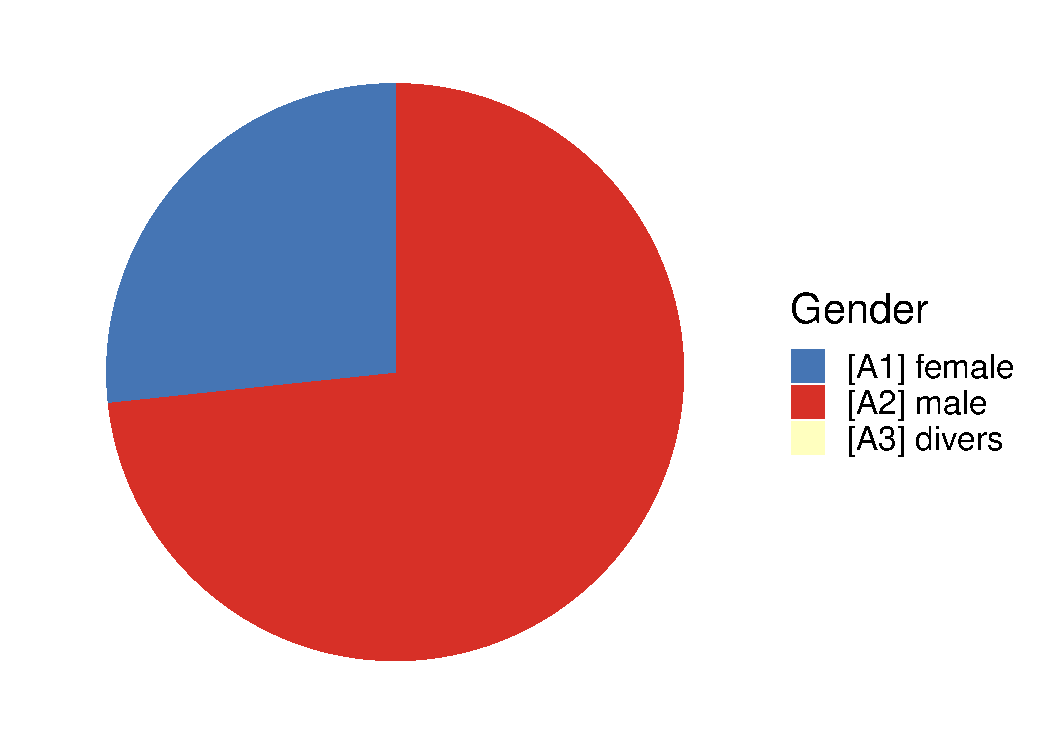
\includegraphics[width=0.75\textwidth]{./appendices/gender}
	\caption{Geschlechterverteilung der Studienteilnehmer}
	\label{fig:gender}
\end{figure}

Das Alter der Teilnehmer reichte von 19 bis 30 Jahren, wobei der Median bei 23 und der Mittelwert bei 23,04 Jahren mit einer Standardabweichung von 2.53 lag. Eine grafische Darstellung kann in Abbildung~\ref{fig:age} und die zugehörigen Zahlenwerte in Tabelle~\ref{tab:sc_results_age} gesehen werden.

\begin{figure}[H]
	\centering
	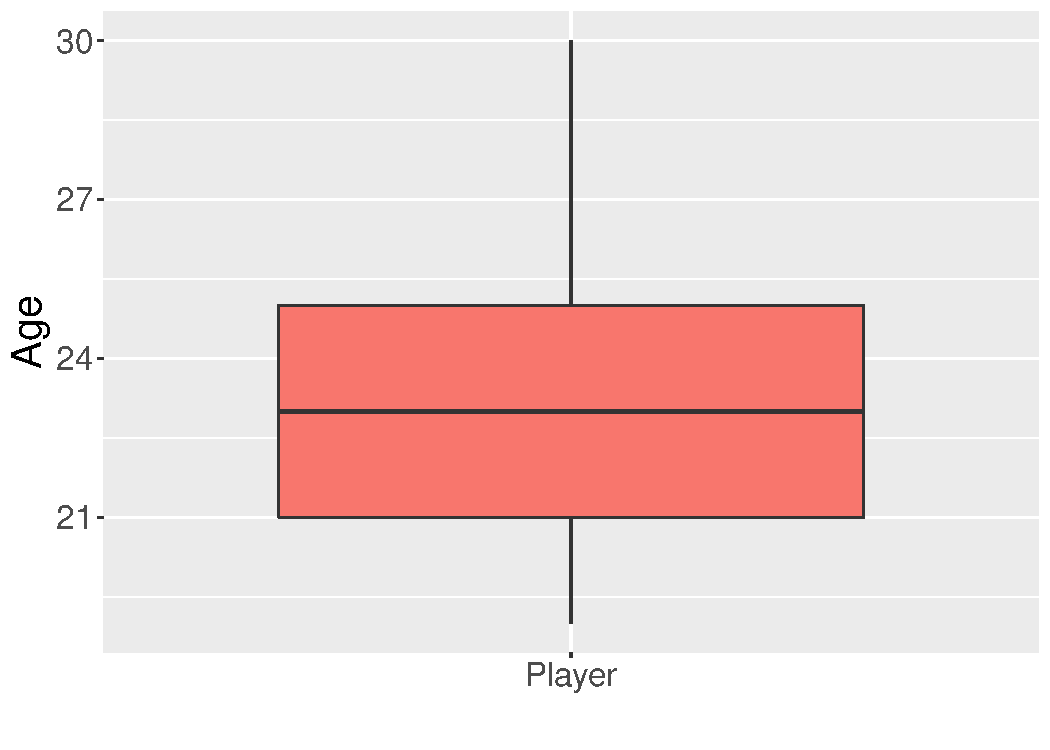
\includegraphics[width=0.75\textwidth]{./appendices/age}
	\caption{Boxplot des Alters der Studienteilnehmer}
	\label{fig:age}
\end{figure}

Die Teilnehmer gaben an, dass sie unterdurchschnittlich wenig Erfahrung mit virtueller Realität haben. Hierbei lag der Mittelwert bei 2,93 von 7 möglichen Punkten. Die Standardabweichung beträgt 1,78. Die Ergebnisse können auch in Tabelle~\ref{tab:sc_results_expVR} und Tabelle~\ref{tab:sc_numbers_expVR} angesehen werden. Bei augmentierter Realität sehen wir ein ähnliches Abbildung. Hier gaben die Teilnehmer an einen durchschnittlichen Erfahrungswert von 2.36 von 7 zu haben. Die Standardabweichung in diesem Fall beträgt 1,38. Außerdem ist noch hervorzuheben, dass keiner der Befragten einen Wert von 7 ausgewählt hat. Die Ergebnisse hierzu können in Tabelle~\ref{tab:sc_results_expAR} und Tabelle~\ref{tab:sc_numbers_expAR} eingesehen werden, zusätzlich existiert eine grafische Repräsentation in den Abbildungen~\ref{fig:expVr} und~\ref{fig:expAr}.

\begin{figure}[H]
	\centering
	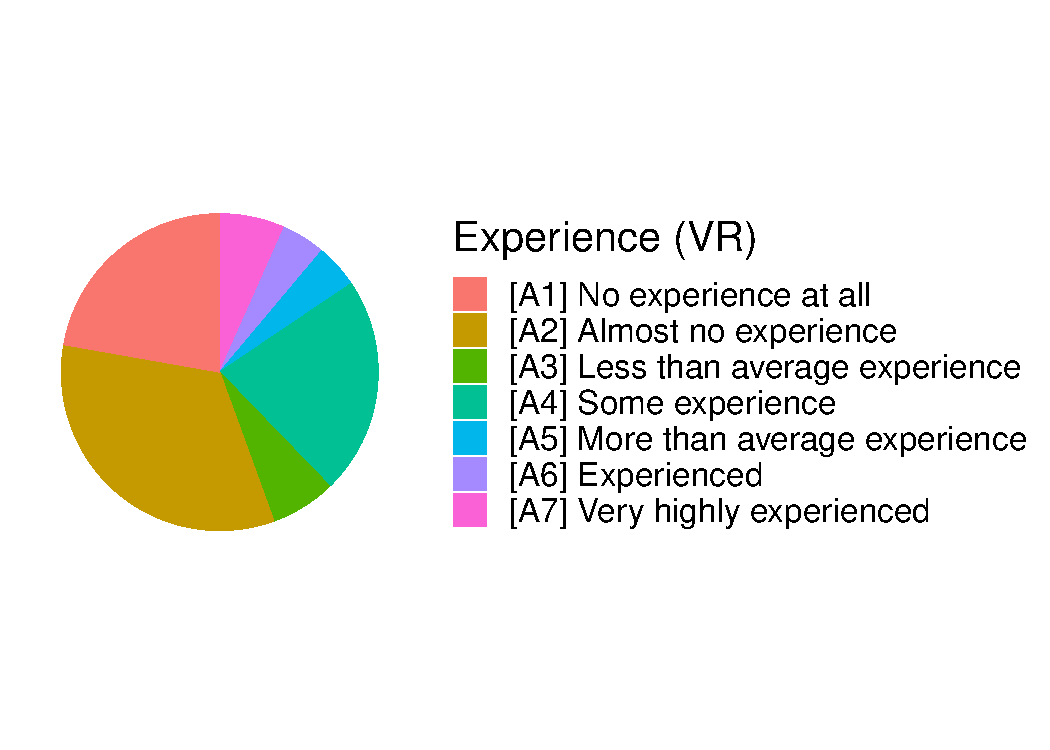
\includegraphics[width=0.75\textwidth]{./appendices/expVr}
	\caption{Grafische Repräsentation der Antworten zur Frage "`How much experience do you have with VR?"'.}
	\label{fig:expVr}
\end{figure}%
\begin{figure}[H]
	\centering
	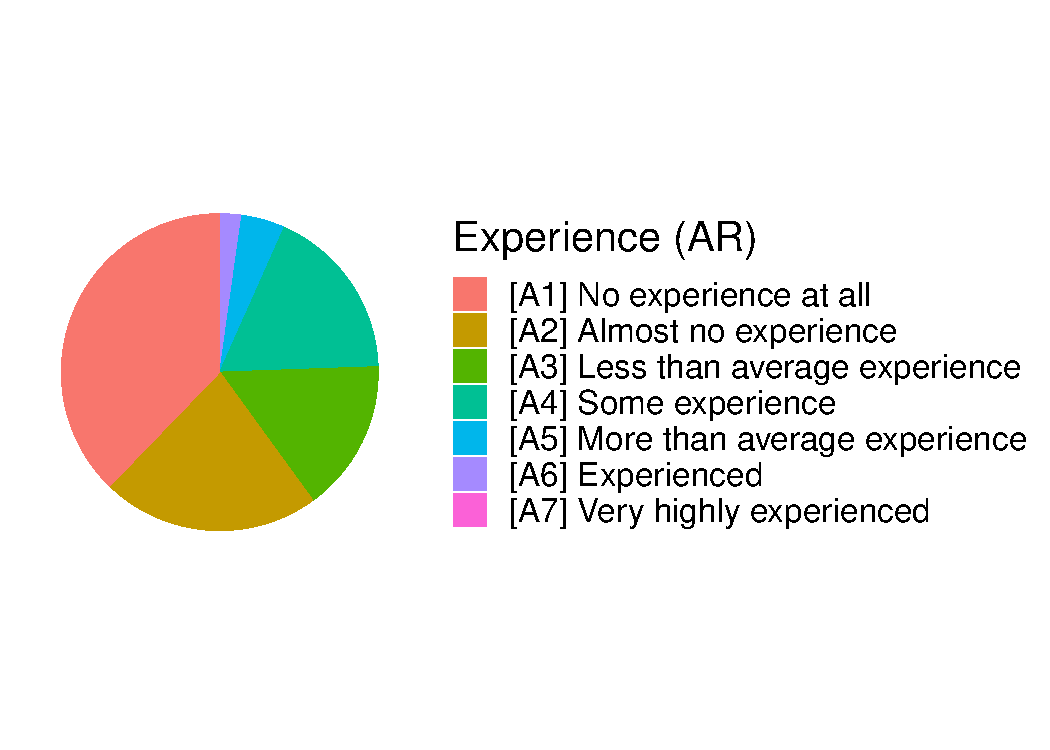
\includegraphics[width=0.75\textwidth]{./appendices/expAr}
	\caption{Grafische Repräsentation der Antworten zur Frage "`How much experience do you have with AR?"'.}
	\label{fig:expAr}
\end{figure}

Das Ausfüllen des SAM Fragebogen wurde einmal vor und einmal nach der Ruhephase verlangt. \todoTob{SAM Ergebnisse beschreiben, zählt SAM zu demografisch?}

\begin{figure}[H]
	\centering
	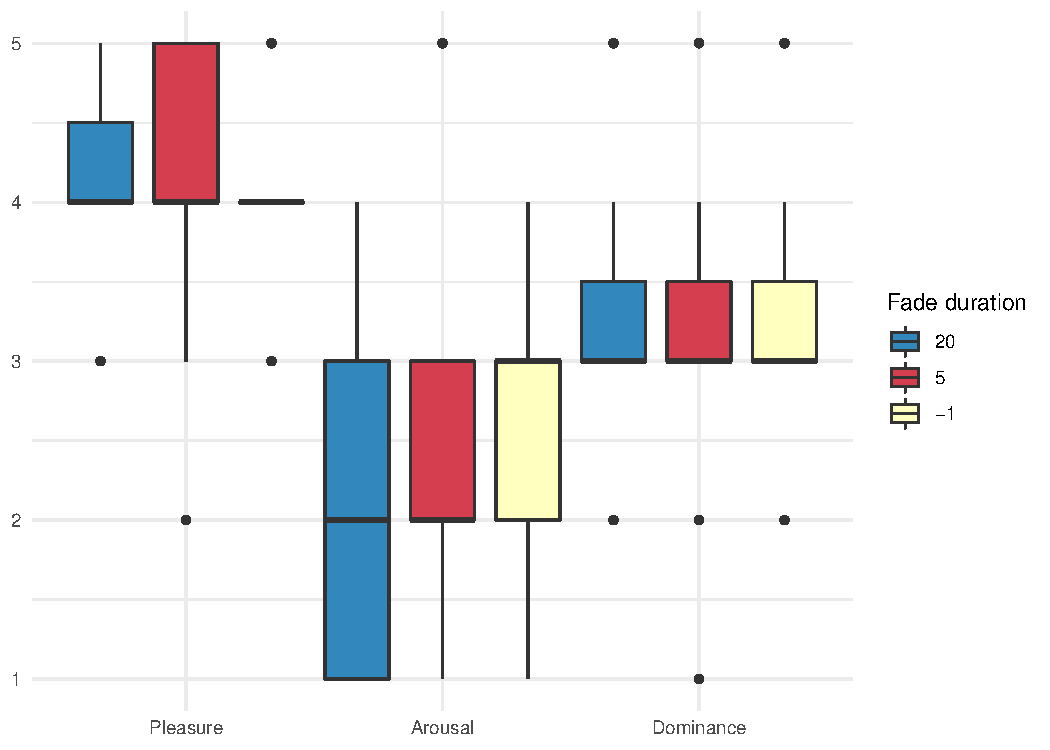
\includegraphics[width=0.75\textwidth]{./appendices/SAMpre}
	\caption{Self-Assessment Manikin Ergebnisse vor der Ruhephase}
	\label{fig:samPre}
\end{figure}%
\begin{figure}[H]
	\centering
	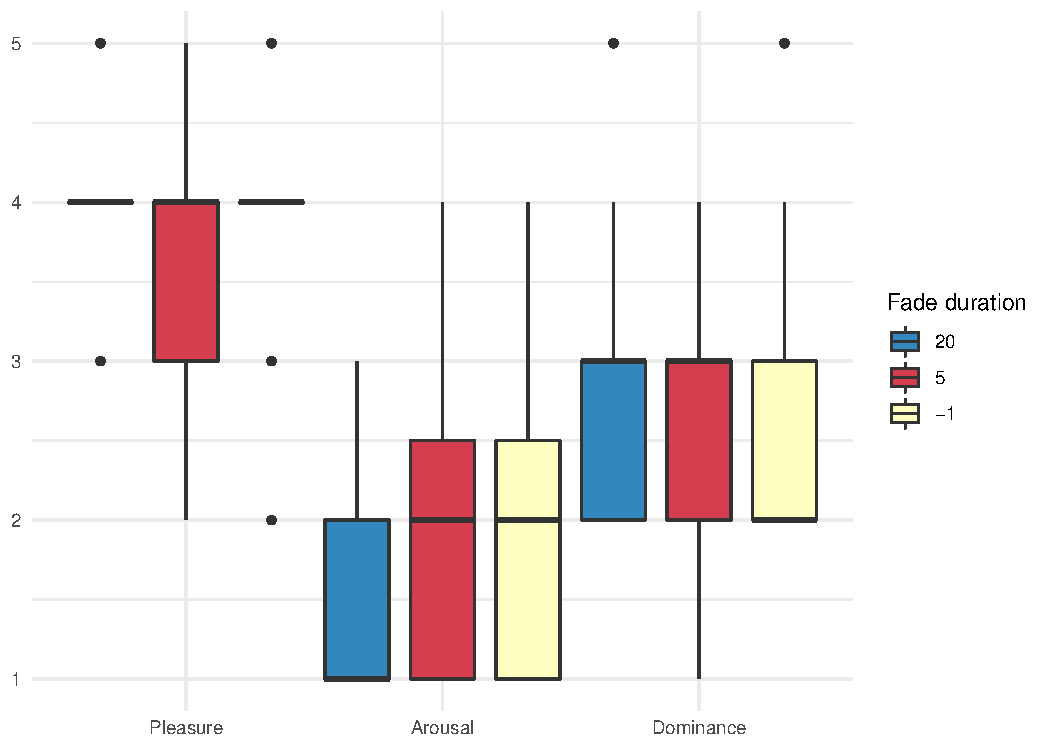
\includegraphics[width=0.75\textwidth]{./appendices/SAMpost}
	\caption{Self-Assessment Manikin Ergebnisse nach der Ruhephase}
	\label{fig:samPost}
\end{figure}


\subsection{Umgebungsvariablen}
Die Umgebung der Studie wurde so abgeschottet gewählt, dass wenig äußere Einflüsse störend auf den Studienablauf wirken konnten. Trotz dieser Platzwahl bekamen wir Rückmeldung durch die Prbanden, dass sie die Umgebung nicht perfekt zum Einschlafen gewählt wurde. Weitere Kommentare der Nutzer zur Bequemlichkeit der VR Brille, als auch zum Stuhl, sowie allen weiteren Umgebumgsvariablen können im Anhang gefunden werden.

Die durchschnittliche Neigung der Stuhllehne lag über alle Durchläufe bei 38,6$^\circ$. Eine genaue Auflistung der Einstellungen kann in Tabelle~\ref{tab:sc_results_chair} eingesehen werden. Hierbei ist zu beachten, dass die Werte vom Studienbetreuer zur Zeit der Ruhephase subjektiv notiert wurden. Außerdem ist zu beachten, dass die Winkeleinstellung mit einer Abweichung notiert worden sein kann. Hierdurch ergeben sich die hier aufgeführten Ergebnisse. Die möglichen Einstellung des verwendeten Stuhls können in Abbildung~\ref{fig:chair_backrest} gefunden werden.

\begin{figure}[H]
	\centering
	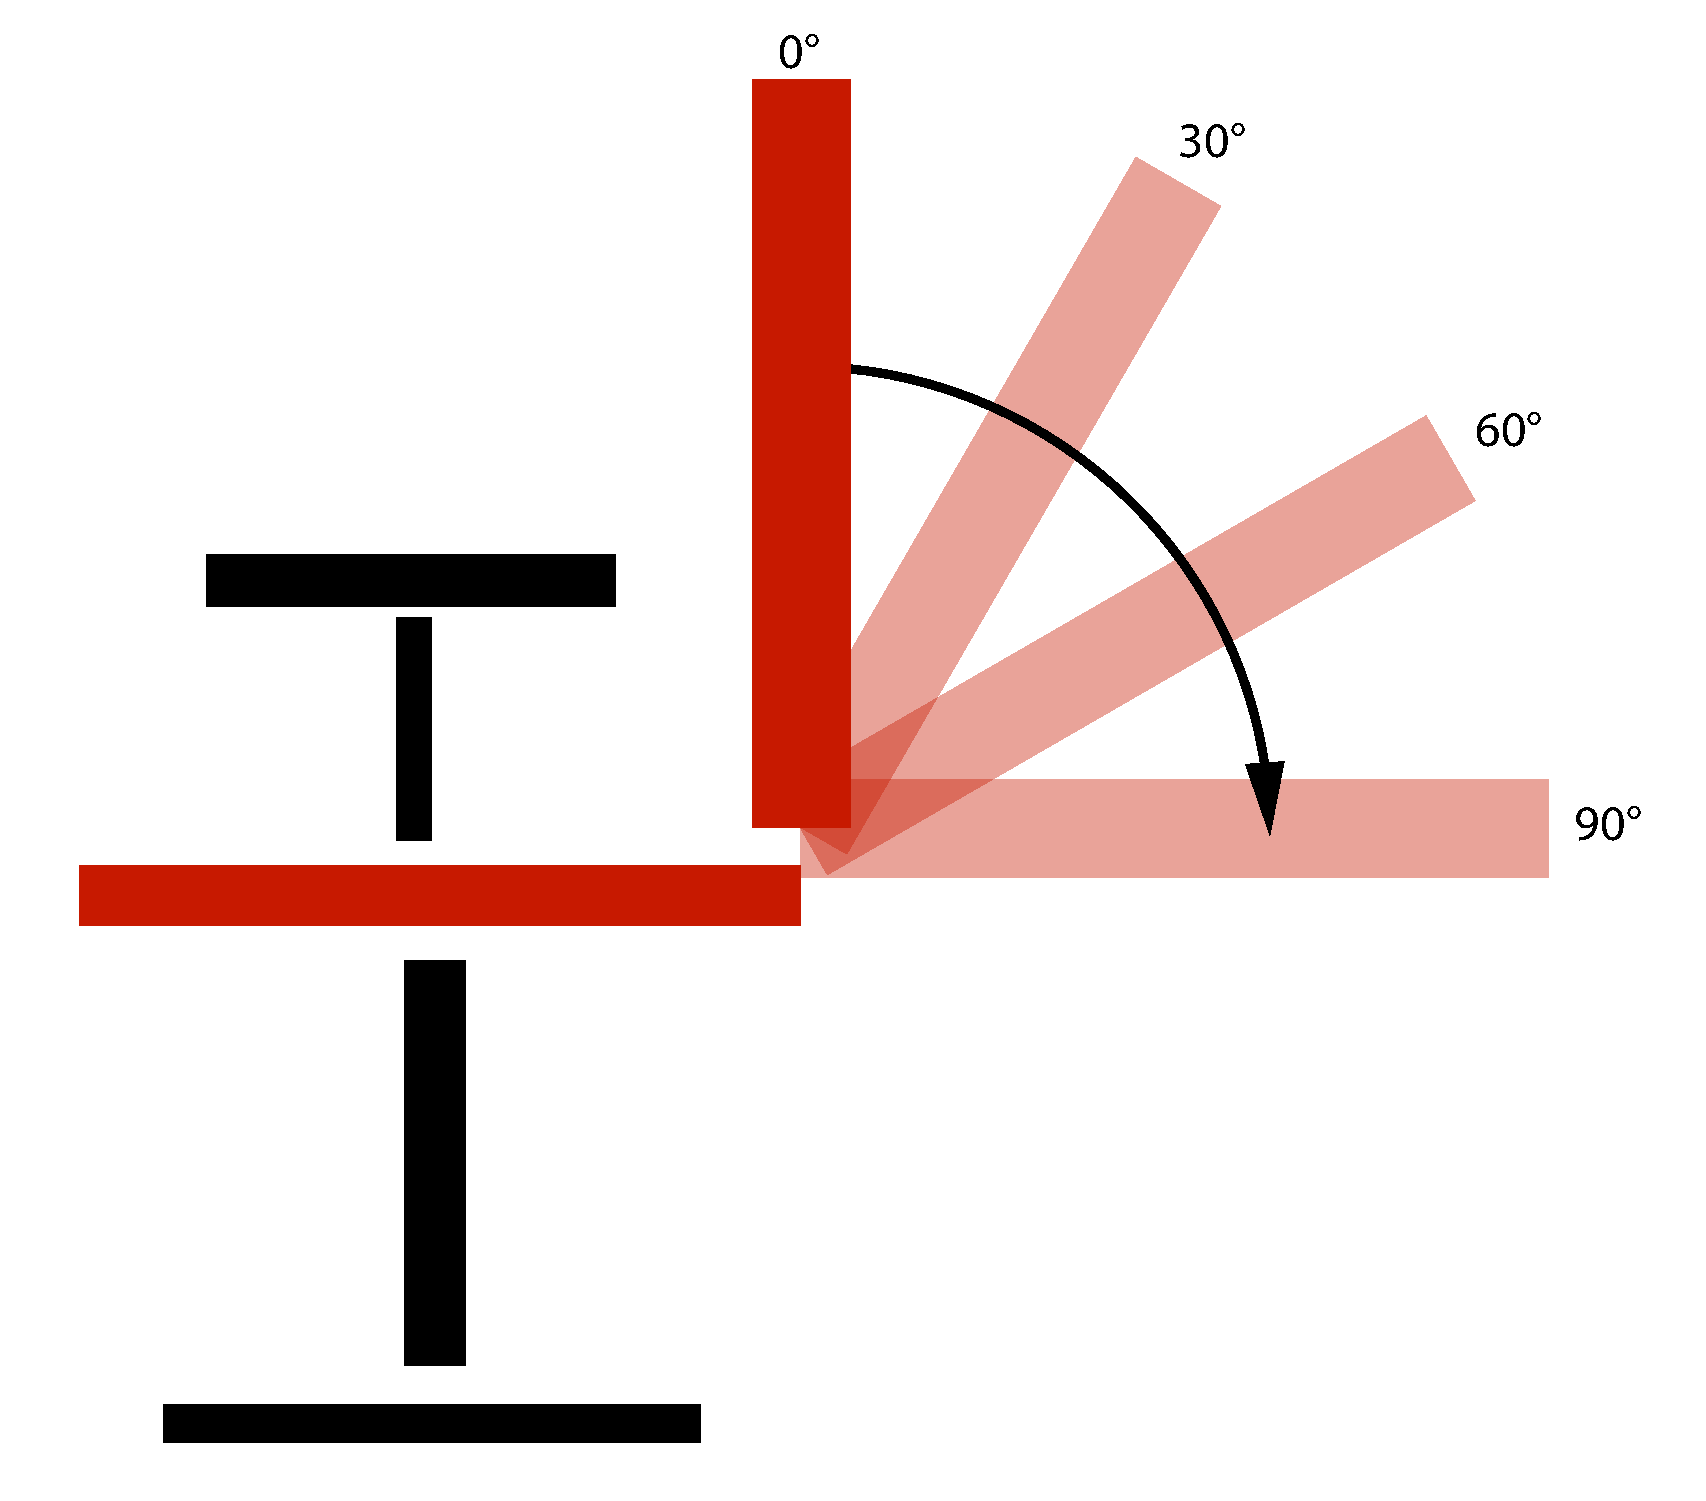
\includegraphics[width=0.75\textwidth]{./images/chair}
	\caption{Winkeleinstellungen vom verwendeten Stuhl in der Studie}
	\label{fig:chair_backrest}
\end{figure}

\subsection{Aufgabenergebnisse} %Fehler, Zeiten, pro Aufgaben
\todoTob{Ergebnisse: Fehlerraten innerhalb der Aufgaben}
\todoTob{Ergebnisse: Zeit für die Erledigung der Aufgaben}
\todoTob{Ergebnisse: Dauer bis Probanden der 2. Studie den Ton abgeschalten haben}

\subsection{Selbsteinschätzungen, Fragebögen} %nur Vorschläge zur Gleiderung; hier sowas wie.. SAM, oder so..?
\todoTob{Ergebnisse: Empfundene Dauer der Ruhephase}
\todoTob{Ergebnisse: RSME Werte}
\todoTob{Ergebnisse: limesurvey zeug}
\todoTob{Ergebnisse: Kopfbewegungen}